\documentclass[a4paper, titlepage]{article}

\usepackage{graphicx}
\usepackage[colorlinks = true]{hyperref}
\usepackage[thinc]{esdiff}
\usepackage{matlab-prettifier}
\usepackage{listings}
\usepackage{cite}
\usepackage{amsmath,amssymb,amsfonts}
\usepackage{algorithmic}
\usepackage{graphicx}
\usepackage{textcomp}
\usepackage{xcolor}
\usepackage{float}
\def\BibTeX{{\rm B\kern-.05em{\sc i\kern-.025em b}\kern-.08em
    T\kern-.1667em\lower.7ex\hbox{E}\kern-.125emX}}
\usepackage{titling}

\title{
    \begin{center}
        \Huge \textbf{Four-Bit ALU}
    \end{center}
    \vspace{0.5cm}
    \textbf{Final Project} - VLSI (EC2.201)\\
}
\author{
    \textbf{Soham Vaishnav}\\ 
    2022112002\\
    \textit{soham.vaishnav@research.iiit.ac.in}
}

\setcounter{section}{0}

\begin{document}

\maketitle
\tableofcontents

\newpage

\section{About ALU}
\textbf{ALU} stands for \textbf{A}rithmetic and \textbf{L}ogic \textbf{U}nit.
As the name suggests, this particular unit in the processor is dedicated to all the tasks
that require basic mathematical operations and also the tasks that require manipulation of data 
using basic binary logic operations. The ALU therefore becomes an extremely crucial component of 
a CPU. \newline 
The structure of an ALU consists of registers, counters and blocks of combinational logic 
that serves as the basis of all the arithmetic and logic operations. The registers are used to 
store the data which latches on to the inputs of the ALU as and when required, and all the flow
of data within the ALU is controlled by a clock. \newline 
One of the most prominant blocks of an ALU is a \textbf{MUX} or a \textbf{Decoder}. This block of 
combinational logic helps in enabling the ALU to compute only the operation that has been asked for
by the user. It does this by keeping a set of \textbf{select lines} that \textit{choose} what function 
to perform. The choice is realised in the form of an \textbf{enable} to that particular arithmetic or 
logic block of combinational logic. A very crude visualisation of an ALU is given in \hyperlink{ALU}{Fig.1}.

\begin{figure}[htp]
\centering
\hypertarget{ALU}{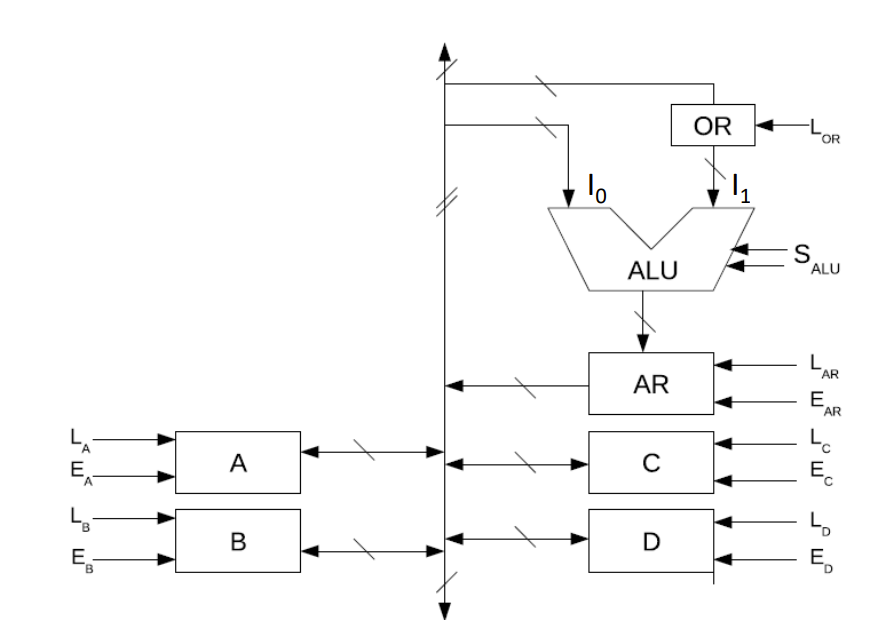
\includegraphics[width=\textwidth]{Image_ALU.png}}
\caption{Basic Design of an ALU}
\label{fig:sysfig}
\end{figure}

\section{Project - Four-bit ALU}
The project aims to impart the knowledge of designing a simple 4-bit ALU that performs operations 
such as Addition, Subtraction, Comparison and ANDing - all applied on two 4-bit numbers. The project
also requires us to perform delay analysis on the operations carried out in order to find 
the maximum or the worst case delay for each of them.\newline 
The tools required to complete the project are - 
\begin{itemize}
    \item \textbf{Verilog} - for logic-level coding 
    \item \textbf{NGSpice} - for coding gate-level netlist
    \item \textbf{MAGIC} - for designing the layout and verify whether the previously designed gate
    netlist complies with the resultant layout.
\end{itemize}

\section{Building the Individual Blocks}
This section deals with the approach taken to build the individual blocks which 
when put together, will result into a 4-bit ALU. The reasoning behind a particular design has also been
discussed alongside.
\subsection{2x4 Decoder and Enabler}
To select a particular function/operation to be performed on the two 4-bit input 
numbers, as discussed, we need either a MUX or a Decoder. \newline
In this project we make use of a \textbf{2x4 Decoder}. We chose this because we have four operations to
perform - Addition, Subtraction, Comparison and ANDing - and to use a MUX for this seems over-usage of 
combinational logic which renders less efficiency. Also, there is no input in the first place except for 
the select lines and therefore the task can also be completed using a simple Decoder as stated. \newline
The functional aspects of the Decoder used here are as follows - 
(Note that the select lines are named as \textbf{Sel0} and \textbf{Sel1})

\begin{table}[h]
\begin{center} 
\hypertarget{dec_tab}{
\begin{tabular}{|c|c|c|}
    \hline 
    \textbf{Sel0} & \textbf{Sel1} & \textbf{Operation} \\
    \hline
    0 & 0 & Addition \\
    \hline 
    0 & 1 & Subtraction \\
    \hline 
    1 & 0 & Comparison \\
    \hline 
    1 & 1 & ANDing \\
    \hline
\end{tabular}}
\caption{Functional aspects of the Decoder}
\label{tab:t1}
\end{center}
\end{table}
Now based on the table above we design the Decoder with the following design - 
\begin{figure}[htp]
    \centering
    \hypertarget{Dec}{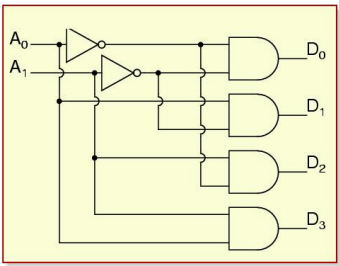
\includegraphics[scale = 0.6]{Image_Decoder.png}}
    \caption{2x4 Decoder}
    \label{fig:fig1}
\end{figure}

Infering from \hyperlink{Dec}{Fig.2}, \textbf{A0} and \textbf{A1} stand for select lines \textbf{Sel0}
and \textbf{Sel1} respectively. Also, logically based on \hyperlink{dec_tab}{Table 1}, \textbf{D0} 
corresponds to \textbf{Addition}, \textbf{D1} to \textbf{Subtraction}, \textbf{D2} to \textbf{Comparison} and 
\textbf{D3} to \textbf{ANDing}. These outputs of the Decoder therefore serve as the \textit{Enables} (\textbf{En}) 
for the functional combinational blocks. \newline 
\textbf{Note} - We will apply the enables to the output of each operational blocks rather than applying it 
to the inputs to those blocks. The reasons are discussed below-
\begin{itemize}
    \item To reduce the number of gates used which will therefore reduce the area of the layout 
    \item By applying enables to the inputs, we will create an issue for the Comparator, especially when it isn't to 
    be used because then all the \textit{effective} inputs to the comparator will be 0 which will basically signal it 
    output a logic high at the \textbf{Eql}, thereby indicating that the inputs are equal, which is what we do not want 
    when other some other block is under use
\end{itemize}

\subsection{Operational Blocks}
In this subsection, we will discuss the designing (combinational logic) of the four functional blocks.
\subsubsection{4-bit Adder/Subtractor}
Basic idea here is to make a common block for carrying out addtion and subtraction simply by a \textit{switching}
mechanism which will be driven by the select lines chosen by the user. Reason behind doing this is to primarily
reduce the repetition of blocks because subtraction for radix-2 numbers is basically adding the 2's compliment 
of the subtrahend to the minuend. \newline 
The mechanism for taking a 2's compliment of an n-bit number is 2-step process-
\begin{itemize}
    \item XOR all the bits with 1 which inverts them 
    \item Add 1 to the resultant number
\end{itemize}
One another design principle that we use for designing a basic adder is making use of full-adders. In our case 
since we are adding two 4-bit numbers, we make use of four full-adders with the first full-adder having a carry \textbf{C0}
as an input and the for the remaining full-adders, the carry to those will be the output carry of the immediate previous 
full-adder. Since we are adding two 4-bit numbers, it is very much likely that we get a 5-bit number as an output, where
the $5^{th}$ bit (or the MSB) will be the output carry of the last full-adder. \newline 
Now, we want this same block to work as an adder or as a subtractor based on the select lines that the user chooses. 
Therefore, based on the subtraction steps discussed earlier and using basic digital logic schemes
we note that if we XOR all bits with 1, they get inverted 
and if we XOR them with 0, they remain the same, and if subtraction is to be performed, we put the first carry as 1 (to get
2's complimentof the subtrahend), otherwise 0. Overall, the first carry will be the bit with which we XOR the bits of the
second number.
\subsubsection{4-bit Comparator}
\subsubsection{4-bit ANDer}
\section{Tools/Platforms used for Building}
explain which tools/platforms were used to build the project
and explain what approach was taken while building those (subckt and subcells)
\subsection{Verilog}
\subsection{Ngspice}
\subsection{MAGIC Layout}
\section{Results and Inference}
state the results - plots and delay analysis and analyse the design and netlist 
of ALU based on the result 
\subsection{Verilog}
\subsection{Ngspice}
\subsection{MAGIC Layout}
\section{Conclusion}
conclude the project
\end{document}